\documentclass[12pt]{article}
\setlength\parindent{0pt}
\usepackage{fullpage}
\usepackage{amsmath}
\usepackage{graphicx}
\setlength{\parskip}{4mm}
\def\LL{\left\langle}   % left angle bracket
\def\RR{\right\rangle}  % right angle bracket
\def\LP{\left(}         % left parenthesis
\def\RP{\right)}        % right parenthesis
\def\LB{\left\{}        % left curly bracket
\def\RB{\right\}}       % right curly bracket
\def\PAR#1#2{ {{\partial #1}\over{\partial #2}} }
\def\PARTWO#1#2{ {{\partial^2 #1}\over{\partial #2}^2} }
\def\PARTWOMIX#1#2#3{ {{\partial^2 #1}\over{\partial #2 \partial #3}} }
\newcommand{\BE}{\begin{displaymath}}
\newcommand{\EE}{\end{displaymath}}
\newcommand{\BNE}{\begin{equation}}
\newcommand{\ENE}{\end{equation}}
\newcommand{\BEA}{\begin{eqnarray}}
\newcommand{\EEA}{\nonumber\end{eqnarray}}
\newcommand{\EL}{\nonumber\\}
\newcommand{\la}[1]{\label{#1}}
\newcommand{\ie}{{\em i.e.\ }}
\newcommand{\eg}{{\em e.\,g.\ }}
\newcommand{\cf}{cf.\ }
\newcommand{\etc}{etc.\ }
\newcommand{\Tr}{{\rm tr}}
\newcommand{\etal}{{\it et al.}}
\newcommand{\OL}[1]{\overline{#1}\ } % overline
\newcommand{\OLL}[1]{\overline{\overline{#1}}\ } % double overline
\newcommand{\OON}{\frac{1}{N}} % "one over N"
\newcommand{\OOX}[1]{\frac{1}{#1}} % "one over X"



\begin{document}
\Large
\centerline{\sc{Homework 6}}
\normalsize
\centerline{\sc{Due before recitation on Friday, April 9}}

{\bf Note: This is a short homework set. Another set of four more challenging problems will be assigned near the middle of next week; they will be due Tuesday, April 13, before Quiz 4. This means that you will have two short homework sets on the conservation of momentum.}

\begin{enumerate}

\item {A train car with a mass of 10,000 kg is rolling slowly down a railway at 0.5 m/s. It encounters another train car with mass 15,000 kg that is parked on the tracks. When the two cars hit each other, they couple together.
	
\begin{enumerate}
	\item How fast are they moving after they couple together?
	\item Suppose that the coefficient of rolling friction between the cars and the tracks is $\mu_r=0.02$. {\it (Rolling friction works just like kinetic friction.)} How far will they roll before they come to a stop? {\it (Hint: You will need to dust off your kinematics and your knowledge of Newton's second law here.)}
\end{enumerate}
}

\item A forensics laboratory is investigating a crime and wants to measure how fast a particular gun shoots bullets. They don't have access to high-speed photography. All they have a clay block sitting on a table.

One of the detectives says ``Hey, we can figure it out using this! We'll set the block on a table and shoot a bullet into the block; the faster the bullet is going, the further the block will slide before it comes to a stop!''

Another detective says ``Yes, we can do that! In addition to how far the block slides on the table, we'll need to measure two things about the block and one thing about the bullet in order to figure it out.''

\begin{enumerate}
	\item What things must they measure to conduct the experiment?
	\item Determine a formula for the speed of the bullet in terms of the other things you measured.
\end{enumerate}

\item{ We return to our astronaut drifting in space. This time, they are using their jet pack to maneuver around a space station to make repairs. They have completed their task, and now want to return to the airlock. Since we have no ``north, south, east, west'' in space, we must create a coordinate system.

Suppose they and their equipment have a mass of 250 kg, and their velocity is currently $\vec v = (1 \rm m/\rm s, 0)$ -- that is, they are moving at 1 m/s in the +x direction. The airlock is located to their side in the +y direction; to reach it, they want to use their jet pack to change their velocity to $\vec v = (0, 0.4 \rm m/\rm s)$. 

If their jet pack exhausts gas at 300 m/s, determine:

\begin{enumerate}
	\item how much gas they need to release, and
	\item which direction they should point the jet pack
\end{enumerate}

in order to change their velocity as they want.
}
\item{In the classic computer game {\it Portal}, the player is asked to solve
	puzzles with the use of a ``portal device'', which can create two connected portals
	on, for example, the floor and a wall. An object entering one portal with speed $v$
	will exit the other with the same speed. Here's an illustration:
	
	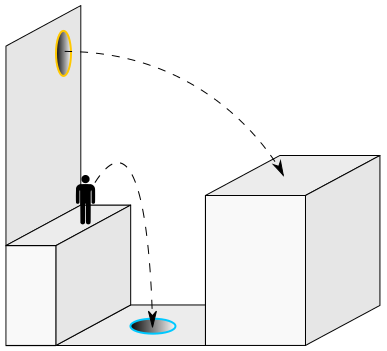
\includegraphics[width=0.4\textwidth]{Portal_physics-2.png}
	
	The game's narrator helpfully explains that ``Forward momentum, a product of mass
	and velocity, is conserved between portals. In layman's terms: {\bf speedy thing
		goes in; speedy thing comes out.}''


Is this an accurate statement of the law of conservation of momentum? As the
		narrator claims, does such a device conserve momentum? If not, why not?

}

\end{enumerate}

\end{document}
